\chapter{Quality Assurance \& Evaluation}

% Explaining how your software was tested (using different datasets or in different environments), statistical evaluation of performance, results of user evaluation questionnaires, etc.

% Not sure if this should be here or in a different section....
\section{Continuous Integration}
Throughout the project, Continuous Integration has been a vital element of the quality assurance process. Travis CI was chosen as the Continuous Integration service to be used for the project, and a CI pipeline was developed at the start of the development process to maintain code quality. The stages of this pipeline include running a linter, unit tests, and functional tests, and can be seen in Figure \ref{fig:ci-pipeline} The CI pipeline runs whenever a Pull Request (PR) is opened on the project's GitHub repository from a feature branch, and all stages of the pipeline must pass before the PR can be merged into the master branch.

\begin{figure}[h!]
  \centering
  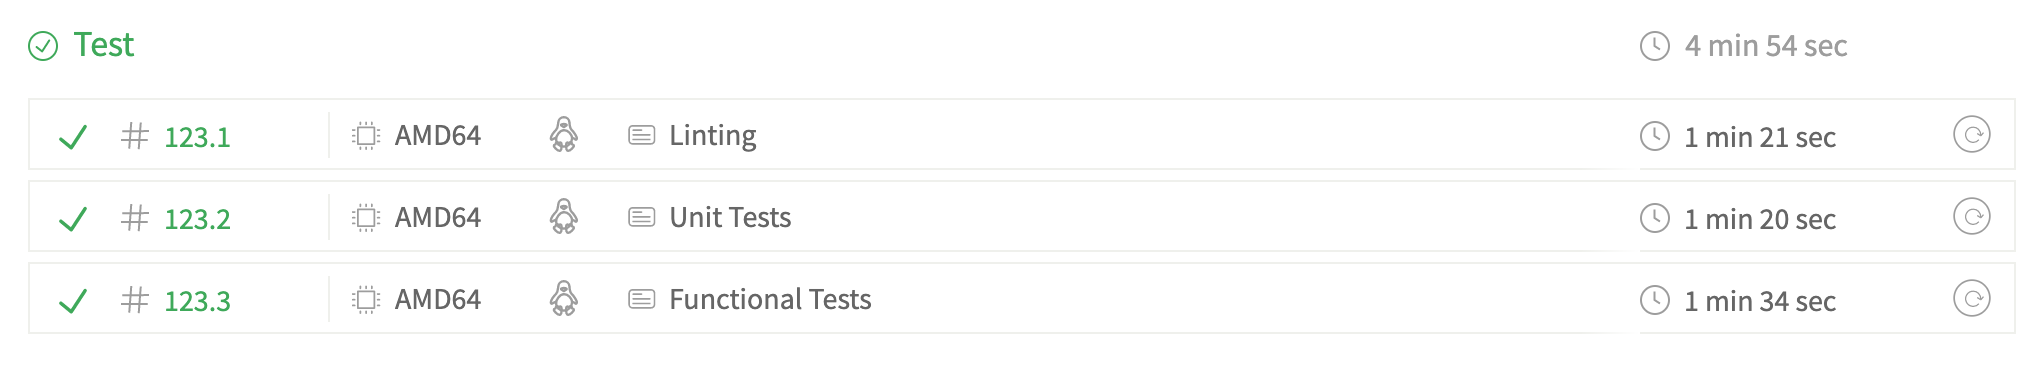
\includegraphics[width=\textwidth]{images/ci-pipeline.png}
  \caption{Continuous Integration pipeline stages on Travis CI}
  \label{fig:ci-pipeline}
\end{figure}

\section{Code Style}
As part of the quality assurance process, it is important that code is written in a consistent style across all areas of the project. The code style for this project is based on the AirBnB JavaScript styleguide, with some modifications to match styles preferred by the Prettier code formatter, in addition to some custom linting rules specific to this project. The style rules are enforced by ESLint, an open-source linter for JavaScript. The full ESLint configuration can be found in the \verb|.eslintrc.json| file in the source repository. By keeping consistent code style, maintenance of the project becomes simplified, and code remains clear to read and understand. It should also be noted, that in the interests of readability and maintainability, the source code is documented inline with comments explaining the purpose of key sections of code.

\section{Unit Testing}
To ensure that the code meets functional requirements and operates as expected, unit tests were written alongside new code throughout the development process. By writing unit tests at the same time as the code, errors can be identified and resolved quickly. 

The unit tests have been written using Jest, an open source test framework for JavaScript. The primary reason why Jest was chosen as the testing framework for this project was due to its Snapshot Testing feature \cite{jest-snapshot}, allowing tests to take a snapshot of a React component's output and then compare all future test runs to this snapshot. This leads to much cleaner test code, which can be written and maintained more easily. In addition, the tests for React components use the Enzyme library for manipulating, traversing, and simulating interaction events on the component output \cite{enzyme}. 

In total, around 200 unit tests were written for this project, focusing on the most important elements of functionality. Line coverage of the unit tests currently sits at 85\%, which increase confidence that the tests are able to reliably identify problems. An example of some of the tests that have been written can be seen in Figure \ref{fig:test-results}. A priority of any future work on this project should be to attempt to increase unit test coverage, specifically in the service side of the application, to increase confidence in the functionality of the code.

\begin{figure}[h!]
  \centering
  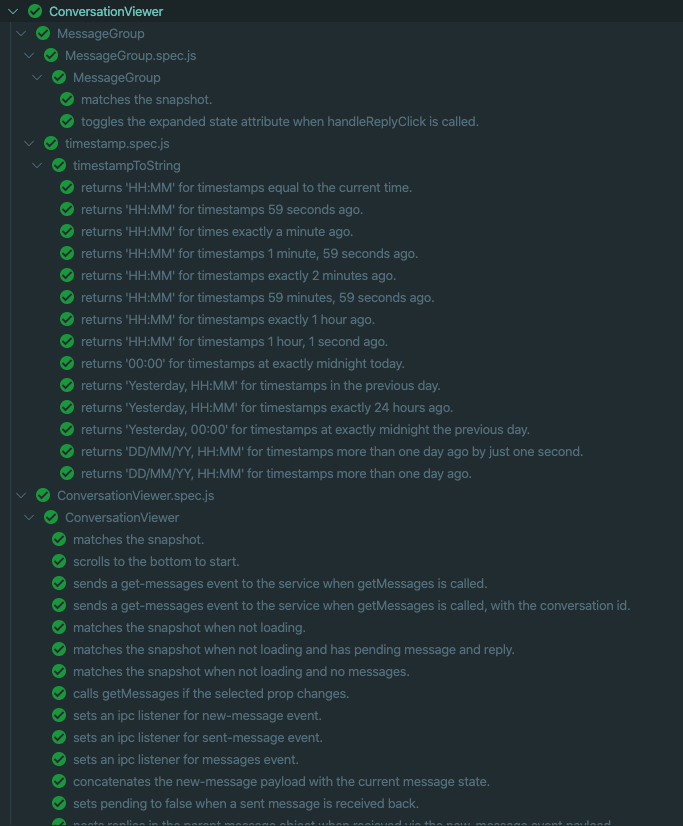
\includegraphics[width=0.7\textwidth]{images/test-results2.png}
  \caption{Example of some of the unit tests written for the software}
  \label{fig:test-results}
\end{figure}

\section{Functional Testing}
In addition to the unit tests described previously, it was intended that this project would make use of automated Functional (End-to-End) tests in order to ensure that the functional requirements of the system are met, as outlined in Section \ref{sec:functional-requirements}. It was decided that Spectron, the de facto tool for automating functional tests for Electron applications would be used to aid in this. However, owing in part to the complexity of the application architecture and build pipeline, some problems were encountered whilst setting up this tooling that took some time to resolve. Not wanting these issues to negatively impact progress, development began alongside working on resolving the issues with Spectron. Whilst the problems were eventually resolved, with a simple test being written as a proof of concept, at this stage a considerable amount of implementation work had been completed, with functional testing being carried out manually. The decision was made that the complex work of writing a backlog of automated functional tests would likely put the project behind schedule. Therefore, functional testing continued to be carried out manually after each feature implementation, with the intention of adding functional tests if time became available. Unfortunately this was not the case, and the writing of automated functional tests is one piece of work that should be considered prior to further work being carried out on the project.


\section{User Acceptance Testing}
In order to assess the quality of the software product, User Acceptance Testing was conducted, where a number of people were asked to use the software to perform a number of tasks whilst under observation, and then answer some questions about the experience. The User Acceptance Testing was planned to take place in two stages:

\begin{enumerate}
  \item First group of users test the software as soon as it is a Minimum Viable Product.
  \item Second group of users test the software at a later stage, once feedback from the first stage has been acted on.
\end{enumerate}

The first stage of this plan was carried out as intended, and the outcomes discussed below, however the second stage of UAT could not be conducted due to the COVID-19 pandemic, which made carrying out observations of users infeasible. Had it taken place, the focus of this stage of UAT would have been to identify whether the issues that arose from the first stage had been sufficiently resolved, as well as testing of additional features. This change of plan really highlights the importance of the Agile development methodology, where testing was not just reserved for the end of the project, and so at least some testing had taken place prior to the pandemic.

\subsection{Stage 1}\label{sec:stage1-uat}
The key objectives of this stage of User Acceptance Testing was primarily to assess the extent to which some of the Non-Functional requirements had been met, which are more difficult to assess through other forms of testing since they are somewhat subjective, but also to ensure that the software works as expected in a real-world environment, including on different operating systems, as users tested the application on their own devices, which included both Windows and MacOS.

% This process stuff should maybe be moved to an appendix...
\subsubsection{Process}

\paragraph{Instructions}
\begin{enumerate}
  \item Install and open the application.
  \item Log in.
  \item Start a new conversation.
  \item Send a message saying `Hi'.
  \item Receive a message.
  \item Reply to the message.
  \item Rename the conversation. 
  \item Receive a message in a new conversation.
  \item Send three messages in the new conversation.
  \item Check the replies to the messages.
\end{enumerate}


\paragraph{Follow-Up Questions}
\begin{enumerate}
  \item How easy did you find the login process?
  \item Were there any frustrating aspects of using the software?
  \item What additional features would you like to see to improve the software?
  \item Did you find the software to be fast and responsive?
  \item Did all aspects of the software behave as you would expect?
  \item Any other comments?
\end{enumerate}

\subsubsection{Key Observations/Feedback}
\begin{itemize}
  \item Immediately maximising the application to be full-screen.
  \item Confusion about the display name when creating a new conversation.
  \item Messages take a long time to appear in the chat after being sent.
  \item Some users struggled to find the `reply' feature.
  \item Most users found changing the conversation name by clicking on the current name to be intuitive.
  \item All users struggled to find where the new direct replies could be found.
  \item Most users said that they would not have known how to find the login credentials for their own email account.
  \item Many users suggested that it should be easier to differentiate who the sender of messages is.
  \item Every user suggested that they would like to be able to send attachments.
\end{itemize}

\subsubsection{Response to UAT}
The results of this phase of user testing were extremely insightful in understanding both the areas where the application was succeeding as well as areas that required improvement. Following the iterative development cycles provided by the Agile methodology, the feedback from user testing was used to feed back directly into the development priorities for the next iteration of work.

It was decided that addressing users' concerns with existing functionality should take priority over the implementation of brand new features. This is in line with the philosophy that it is much easier and faster to fix issues with software as early as possible, and that making these changes at a later stage in the development process could lead to more work being required unnecessarily. Based on this, a list of feedback-based development priorities was created to direct further development work:

\begin{itemize}
  \item Improve the login process so that common email providers can be used without the need for mail server settings.
  \item Display sent messages in the chat immediately, with a sending indicator until the transport process has completed.
  \item Make new messages more obvious.
  \item Add coloured indicators next to messages to indicate which user sent them.
\end{itemize}